\chapter{Sorting}
\label{chap:sorting}

\section{The sorting problem}
\begin{definition}
    Suppose we have an array $A$. Then we need to find a sorting algorithm such that
    \begin{itemize}
        \item the resulting array is a permutation of $A$ (let's denote this as $S$), and
        \item the resulting array is in nondecreasing order. That is, it satisfies
    \[
    S[1] \le S[2] \le \cdots \le S[n-1] \le S[n].
    \]
    \end{itemize}
\end{definition}

A sorting algorithm can possess certain properties. Of interest for this course are the \textit{stable} property and the \textit{in-place} property.

\begin{definition}
    A sorting algorithm is stable if in case of ties, the relative order of elements is preserved in the resulting sorted array.
\end{definition}

\psset{inline=boxed}
If we were to sort, for example, five playing cards in order of increasing rank (or face value)
\begin{center}
    \crdnines\crdQd\crdfourh\crdsixc\crdfours
\end{center}
then a stable sorting algorithm should output a permutation such that it preserves the relative order between the four of hearts and the four of spades, as shown below.
\begin{center}
    \crdfourh\crdfours\crdsixc\crdnines\crdQd
\end{center}

\begin{definition}
    A sorting algorithm is in-place if it does not use additional data structures while sorting, aside from temporary variables. More precisely, it only consumes $\bigO{1}$ auxiliary space.
\end{definition}

\section{Quadratic-time sorting}
\subsection{Selection sort}
Here's a straightforward way of sorting elements in an array: we find the smallest element and put it in front, then we find the second smallest element and put it in the second position, then we find the third smallest element and put it in the third position, and so on until we reach the last element. This is how \textit{selection sort} works.

In other words, we incrementally build the sorted array by selecting the smallest, then the second smallest, then the third smallest, and so on. So we can say that at the start of $i$th iteration, the first $i-1$ elements are in sorted order, and actually this is the loop invariant for selection sort.

The following algorithm implements selection sort using loops.

\begin{algorithm}[H]
    \caption{An iterative implementation of selection sort}
    \begin{algorithmic}[1]
        \Require An array $A$ of $n$ elements
        \Ensure The array $A$ in sorted order
        \Function{SelectionSort}{$A$}
        \For{$i \gets 1$ to $n-1$}
            \State $k \gets i$
            \Comment{set first unsorted element as current minimum}
            \For{$j \gets i+1$ to $n$}
                \If{$A[j] < A[k]$}
                    \State $k \gets j$
                \EndIf
            \EndFor
            \State \Call{Swap}{$A[i]$, $A[k]$}
            \Comment{put $A[k]$ in the $i$th position}
        \EndFor
        \Return $A$
        \EndFunction
    \end{algorithmic}
\end{algorithm}

What's the running time of selection sort? The outer loop has $n$ iterations, so it contributes $\bigO{n}$ time. The inner loop has \textit{at most} $n-1$ iterations (when $j=1$), so it runs in $\bigO{n}$ time. Since the inner loop is executed at every iteration of the outer loop, then the total running time is $\bigO{n^2}$.

Based from the loop invariant, we can also conclude that if the first $i$ elements are sorted, then the remaining $n-i$ elements are still unsorted. So if we only have the first element sorted, then the remaining elements are not yet sorted. From this insight, we can derive another way of doing selection sort. 

The first step would be to find the smallest element and put that in front. What do we do with the remaining elements? We just sort them by wishfully thinking that you already have a way to sort, and somehow this involves doing a recursive call. 

\begin{algorithm}[H]
    \caption{A recursive implementation of selection sort}
    \begin{algorithmic}[1]
        \Require An array $A$ of $n$ elements
        \Ensure The array $A$ in sorted order
        \Function{SelectionSort}{$A$}
            \If{$n = 1$}
                \Return $A$
                \Comment{sorted by default}
            \EndIf
            \State $k \gets 0$
            \For{$i \gets 1$ to $n-1$}
                \If{$A[i] < A[k]$}
                    \State $k \gets i$
                \EndIf
            \EndFor
            \State \Call{Swap}{$A[0]$, $A[k]$}
            \Comment{put minimum element in front}
            \Return \Call{Cons}{\Call{First}{$A$}, \Call{SelectionSort}{\Call{Rest}{$A$}}}
        \EndFunction
    \end{algorithmic}
\end{algorithm}

Would a recursive implementation be better in terms of running time? Let $T\left(n\right)$ be the running time of selection sort with input size $n$. Since the base case only returns the array itself, it just runs in constant time so $T\left(1\right) = \bigO{1}$. In the recursive case, the loop to find the minimum element contributes $\bigO{n}$ time, and since we make a recursive call to sort the remaining $n-1$ elements, we get the recurrence $T\left(n\right) = T\left(n-1\right) + \bigO{n}$. Solving this recurrence, we get $T\left(n\right) = \bigO{n^2}$. 

Thus selection sort runs in $\bigO{n^2}$ time regardless if the implementation is iterative or recursive.

\subsection{Insertion sort}
Insertion sort draws inspiration from the way card players arrange the cards in their hands.

\begin{figure}[H]
    \centering
    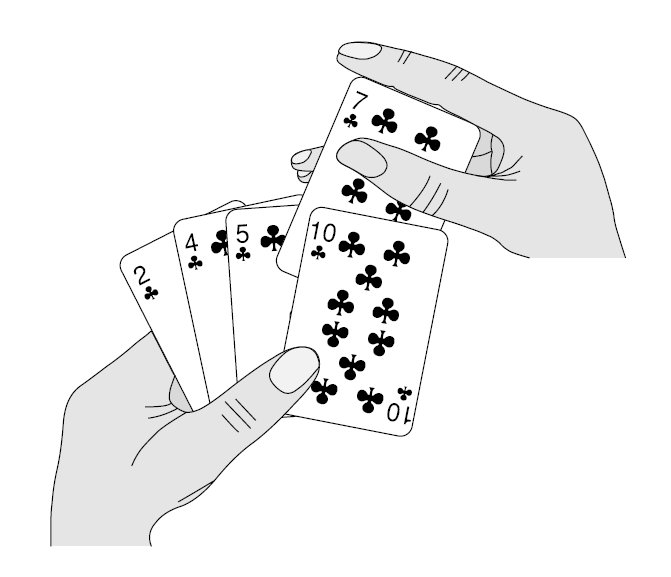
\includegraphics[height=5cm]{figures/insertionsort.jpg}
    \caption{Insertion sort in real life, from \cite{cormen_introduction_2009}}
\end{figure}

\begin{algorithm}[H]
    \caption{An iterative implementation of insertion sort}
    \begin{algorithmic}[1]
        \Require An array $A$ of $n$ elements
        \Ensure The array $A$ in sorted order
        \Function{InsertionSort}{$A$}
        \Statex
        \Comment{mark first element as sorted}
        \For{$i \gets 2$ to $n$}
        \Comment{$i$ is the index of first unsorted element}
            \For{$j \gets i-1$ downto $1$}
            \Comment{try inserting $A[i]$}
                \If{$A[j] > A[j+1]$}
                    \State \Call{Swap}{$A[j]$, $A[j+1]$}
                    \Comment{move sorted element to the right}
                \Else
                    \Break
                    \Comment{insert $A[j+1]$ in position $j$}
                \EndIf
            \EndFor
        \EndFor
        \Return $A$
    \EndFunction
    \end{algorithmic}
\end{algorithm}

\begin{claim}
    The running time of insertion sort is $\bigO{n}$ in the best case, and $\bigO{n^2}$ in the worst case.
\end{claim}
\begin{proof}
    The outer loop has $n-1$, so it contributes $\bigO{n}$ time. For the inner loop, we have two cases.

    The first case is when a swap is due to happen. This means that the inner loop can have at most $n-1$ iterations. Consider when would the inner loop have exactly $n-1$ iterations. This would happen if each consecutive pair of elements in the array have been swapped. This implies that the array must be in reverse sorted order, and we consider this to be the worst case for insertion sort. Therefore the inner loop contributes $\bigO{n}$ time for the worst case.

    The second case is when no swaps will occur. This means that the inner loop terminates after just one iteration. If no elements needed to be swapped, then we can say that the array is already in sorted order, which we consider to be the best case. Therefore the inner loop contributes $\bigO{1}$ time for the best case.

    Since the inner loop is executed at every iteration of the outer loop, then the total running time of insertion sort is $\bigO{n}$ in the best case, and $\bigO{n^2}$ in the worst case.
\end{proof}

\subsection{Bubble sort}

Bubble sort is the conceptually simplest among the quadratic-time sorting algorithms. The main idea behind it is that for every consecutive pair of elements, swap them if they are not in order. Then repeat this process until no more pairs are out of order.

\begin{algorithm}[H]
    \caption{An iterative implementation of bubble sort}
    \begin{algorithmic}[1]
        \Require An array $A$ of $n$ elements
        \Ensure The array $A$ in sorted order
        \Function{BubbleSort}{$A$}
        \Repeat
            \State $\text{swapped} \gets \algfalse$
            \For{$i \gets 2$ to $n-1$}
                \If{$A[i-1] > A[i]$}
                    \State \Call{Swap}{$A[i-1]$, $A[i]$}
                    \State $\text{swapped} \gets \algtrue$
                \EndIf
            \EndFor
        \Until{$\text{swapped} = \algfalse$}
        \Return $A$
        \EndFunction
    \end{algorithmic}
\end{algorithm}

\begin{claim}
    The running time of bubble sort is $\bigO{n}$ in the best case, and $\bigO{n^2}$ in the worst case.
\end{claim}
\begin{proof}
    The best case happens when the array is already sorted. If so, then no swaps are needed, thus the swapped flag stays false. Because of this, the outer loop terminates after one iteration. The inner loop has $n-2$ iterations, so it runs in $\bigO{n}$ time. Then the best-case running time of bubble sort is $\bigO{n}$.

    On the other hand, the worst case happens when the array is in reverse sorted order. Notice that to move the largest element to the last position, $n-1$ swaps are needed. Then to move the second largest element to the second last position, $n-2$ swaps are needed, and so on. So the outer loop will have $n-1$ iterations, thus it runs in $\bigO{n}$ time.

    The inner loop still has $n-2$ iterations. Therefore, the worst-case running time of bubble sort is $\bigO{n^2}$.
\end{proof}

\section{Linearithmic-time sorting}
\subsection{Merge sort}
\subsection{Quick sort}

\section{Lower bounds of sorting}

\section{Linear-time sorting}
\subsection{Bucket sort}
\subsection{Counting sort}
\subsection{Radix sort}

